\documentclass[12pt]{beamer}
\usepackage{cmap}
\usepackage[T2A]{fontenc}
\usepackage[utf8]{inputenc}
\usepackage{ifluatex}
\usefonttheme[onlymath]{serif}
\usepackage{svg}
\usepackage{enumerate}
\usepackage{hyperref}
\usepackage{mathtools}
\setbeamertemplate{footline}[frame number]
\definecolor{beamer@darkgreen}{rgb}{0,0.6,0}
\setbeamercolor{normal text}{fg=black,bg=white}
\setbeamercolor{title}{fg=black,bg=beamer@darkgreen}
\setbeamercolor{frametitle}{fg=black,bg=beamer@darkgreen}
\setbeamercolor{background canvas}{parent=normal text}

\usepackage[english,russian]{babel}
\usepackage{graphicx}
\usepackage{listings}
\DeclareMathOperator{\sign}{sign}

\author{Катя Тузова}
\title{Машинное обучение}
\subtitle{Лекция 6. Метод опорных векторов.}
\date{}

\begin{document}	
\frame{\titlepage}

\begin{frame}\frametitle{Разбор летучки}
\end{frame}

\begin{frame}\frametitle{Постановка задачи}
$X = \mathbb{R}^n$, ${Y = \left\{ -1, + 1\right\}}$\\
${X^l = (x_i, y_i)_{i = 1}^l}$ -- обучающая выборка\\
\vspace{5mm}Найти:\\
$(n-1)$-мерную гиперплоскость, которая разделяет данные как можно лучше.
\\ \vspace{5mm}
Как можно лучше -- это как?

\end{frame}

\begin{frame}\frametitle{Пример}
\begin{figure}[htbp]
  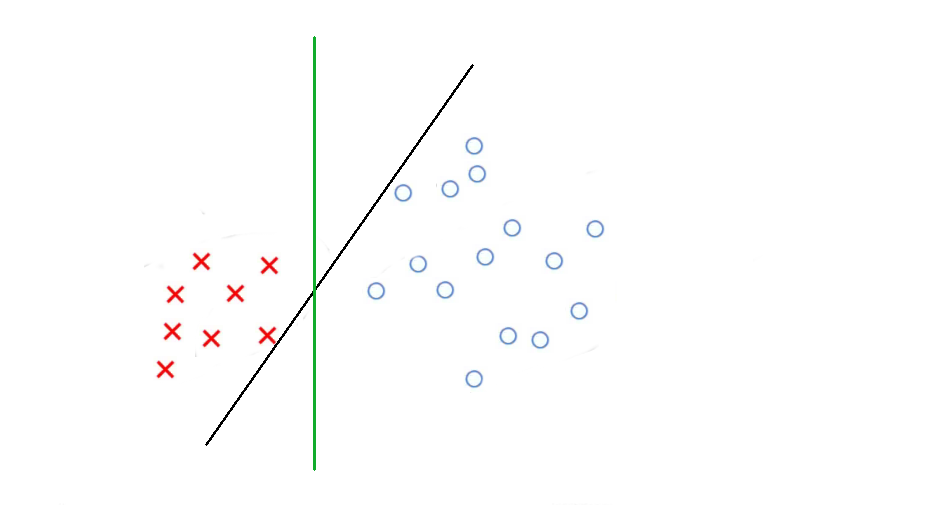
\includegraphics[height=190pt, keepaspectratio = true]{images/example}   
\end{figure}
\end{frame}

\begin{frame}\frametitle{Постановка задачи}
Как можно лучше:\\
Два разделенных класса должны лежать как можно дальше от разделяющей гиперплоскости.\\
\end{frame}

\begin{frame}\frametitle{Опорная гиперплоскость}
\end{frame}

\begin{frame}\frametitle{Опорная гиперплоскость}
Гиперплоскость называется опорной для множества точек
$X$, если все точки из $X$ лежат по одну сторону от этой гиперплоскости.\\\vspace{5mm}
${f(x,w) = \langle x, w\rangle - w_0 = 0}$\\
\vspace{5mm}
Как посчитать расстояние от точки до гиперплоскости?
\end{frame}

\begin{frame}\frametitle{Опорная гиперплоскость}
Гиперплоскость называется опорной для множества точек
$X$, если все точки из $X$ лежат по одну сторону от этой гиперплоскости.\\\vspace{5mm}
${f(x,w) = \langle x, w\rangle - w_0 = 0}$\\
\vspace{5mm}
Расстояние от точки до гиперплоскости:
$\frac{\vert f(x,w) \vert}{\Vert w \Vert}$
\end{frame}

\begin{frame}\frametitle{Максимизиция отступа}
Идея:\\
Максимизировать отступ между двумя параллельными опорными плоскостями, а затем провести параллельную им плоскость на равных расстояниях.\\
\end{frame}

\begin{frame}\frametitle{Постановка задачи}
${X^l = (x_i,y_i)_{i = 1}^l}$\\ 
${Y=\left\{-1,+1\right\}}$\\
\vspace{5mm}
$a(\mathbf{x}, \mathbf{w}) = sign(\langle \mathbf{w}, \mathbf{x}\rangle)$\\
\end{frame}


\begin{frame}\frametitle{Линейно разделимая выборка}
\end{frame}

\begin{frame}\frametitle{Линейно разделимая выборка}
$\exists \mathbf{w}: M_i(\mathbf{w}) = y_i(\mathbf{w}, \mathbf{x_i}) > 0$, i=1, \dots , l\\
\end{frame}

\begin{frame}\frametitle{Линейно разделимая выборка}
\begin{figure}[htbp]
  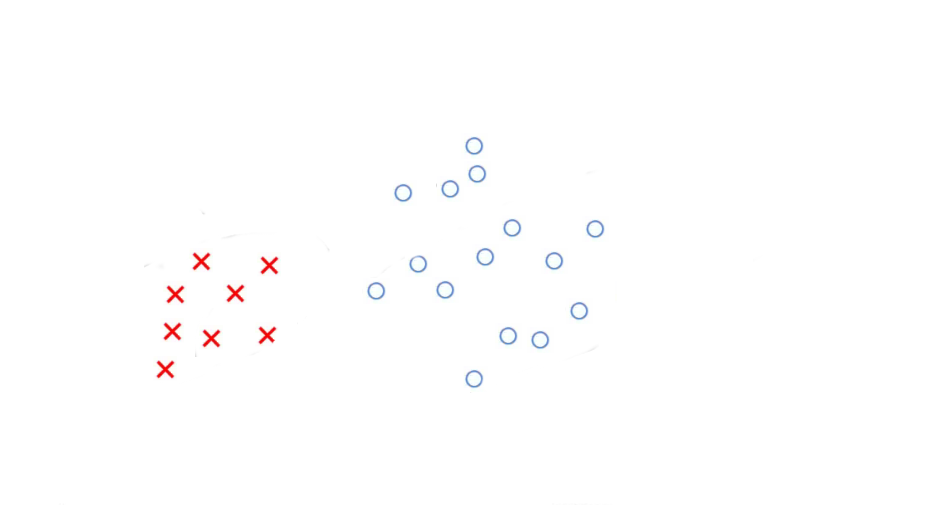
\includegraphics[height=190pt, keepaspectratio = true]{images/linearly_separable1}   
\end{figure}
\end{frame}

\begin{frame}\frametitle{Линейно разделимая выборка}
\begin{figure}[htbp]
  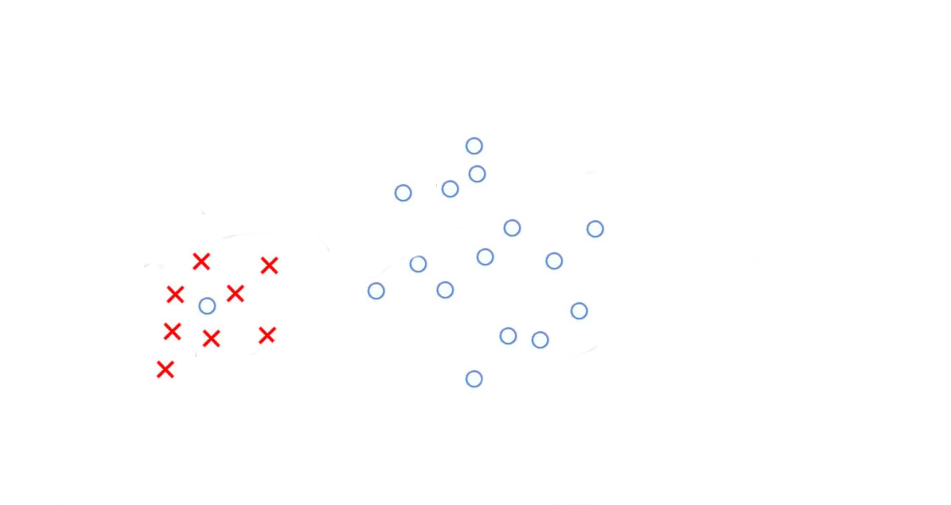
\includegraphics[height=190pt, keepaspectratio = true]{images/linearly_unseparable}   
\end{figure}
\end{frame}

\begin{frame}\frametitle{Оптимальная разделяющая гиперплоскость}
Нормировка: $\min\limits_{i = 1, \dots , l} M_i(\mathbf{w}) = 1$\\
Как выглядит разделяющая полоса?
\begin{figure}[htbp]
  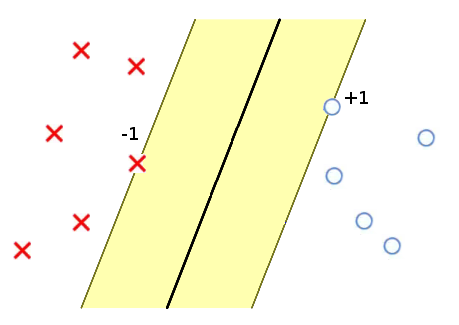
\includegraphics[height=100pt, keepaspectratio = true]{images/linearly_separable3}   
\end{figure}
\end{frame}


\begin{frame}\frametitle{Оптимальная разделяющая гиперплоскость}
Нормировка: $\min\limits_{i = 1, \dots , l} M_i(\mathbf{w}) = 1$\\
Разделяющая полоса: $\left\{\mathbf{x}: -1 \leq \langle \mathbf{w}, \mathbf{x}\rangle \leq 1\right\}$
\begin{figure}[htbp]
  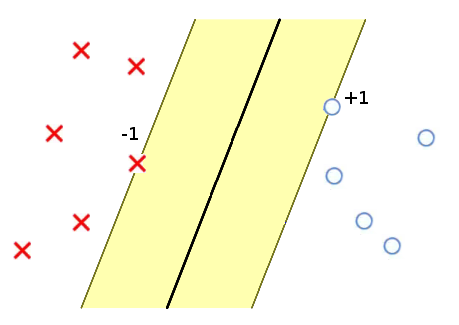
\includegraphics[height=100pt, keepaspectratio = true]{images/linearly_separable3}   
\end{figure}
\end{frame}

\begin{frame}\frametitle{Оптимальная разделяющая гиперплоскость}
Разделяющая полоса: $\left\{\mathbf{x}: -1 \leq \langle \mathbf{w}, \mathbf{x}\rangle \leq 1\right\}$\\
Ширина разделяющей полосы?
\begin{figure}[htbp]
  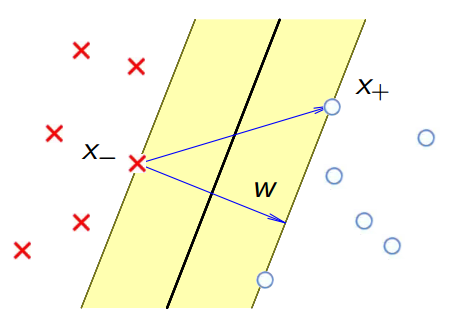
\includegraphics[height=100pt, keepaspectratio = true]{images/linearly_separable}   
\end{figure}
\end{frame}

\begin{frame}\frametitle{Оптимальная разделяющая гиперплоскость}
Разделяющая полоса: $\left\{\mathbf{x}: -1 \leq \langle \mathbf{w}, \mathbf{x}\rangle \leq 1\right\}$\\
Ширина разделяющей полосы: $\frac{\langle \mathbf{x_{+}} - \mathbf{x_{-}, \mathbf{w}} \rangle}{\Vert \mathbf{w} \Vert} = \frac{2}{\Vert \mathbf{w} \Vert} \rightarrow \max$
\begin{figure}[htbp]
  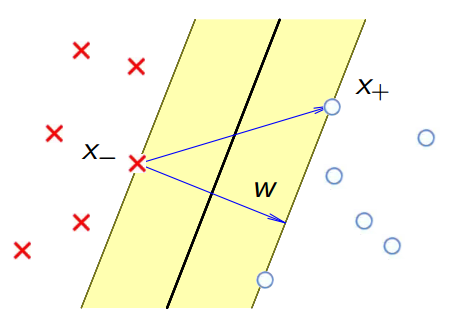
\includegraphics[height=100pt, keepaspectratio = true]{images/linearly_separable}   
\end{figure}
\end{frame}

\end{document}
